\documentclass[aspectratio=1610]{beamer}

\usetheme{metropolis}

\usepackage[russian]{babel}
\usepackage{polyglossia}
\setdefaultlanguage{russian}
\setmainfont{Arial}
\setromanfont{Times New Roman}
\setsansfont{Arial}
\setmonofont{Courier New}

\usepackage{fontspec}
\setmainfont{Times New Roman}
\newfontfamily{\cyrillicfont}{Times New Roman}
\newfontfamily{\cyrillicfontrm}{Times New Roman}
\newfontfamily{\cyrillicfontsf}{Arial}
\newfontfamily{\cyrillicfonttt}{Courier New}

\usepackage{minted}
\setminted{fontsize=\small,baselinestretch=1}

\usepackage{graphicx}
\graphicspath{{../pictures/}{example/}}
\DeclareGraphicsExtensions{.pdf,.png,.jpg}

\usepackage{tikz}
\usetikzlibrary{automata,arrows,chains,shapes.geometric,positioning,calc}

\usepackage{forloop}
\newcounter{example}

\title[Thesis]{Исследование возможности добавления палитры команд
в произвольные приложения\\c использованием фреймворка Qt}
\author{Студент: Польшаков Д.В. \\
Научный руководитель: к.ф.-м.н., доц. Чернышов М.К.}
\institute{ВГУ}
\date{\the\year}

\begin{document}

\begin{frame}[plain]
	\titlepage
\end{frame}

\begin{frame}{Палитра команд}
	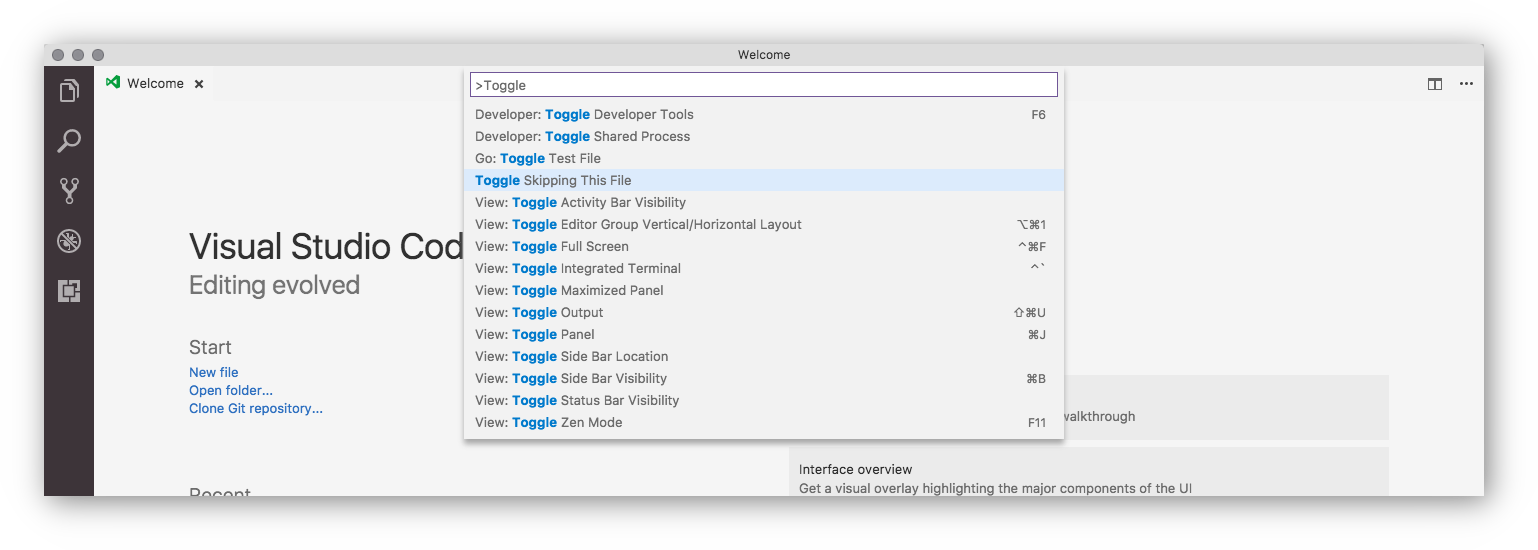
\includegraphics[width=\textwidth]{vscode}
\end{frame}

\begin{frame}{Цель работы}
	\begin{itemize}
		\item Поиск способа добавления новых возможностей\\
		в собранное	ранее приложение
		\item Реализовать систему для добавления палитры команд\\
		в собранное ранее приложение
	\end{itemize}
\end{frame}

\begin{frame}{Палитра команд в Plotinus}
	\centering
	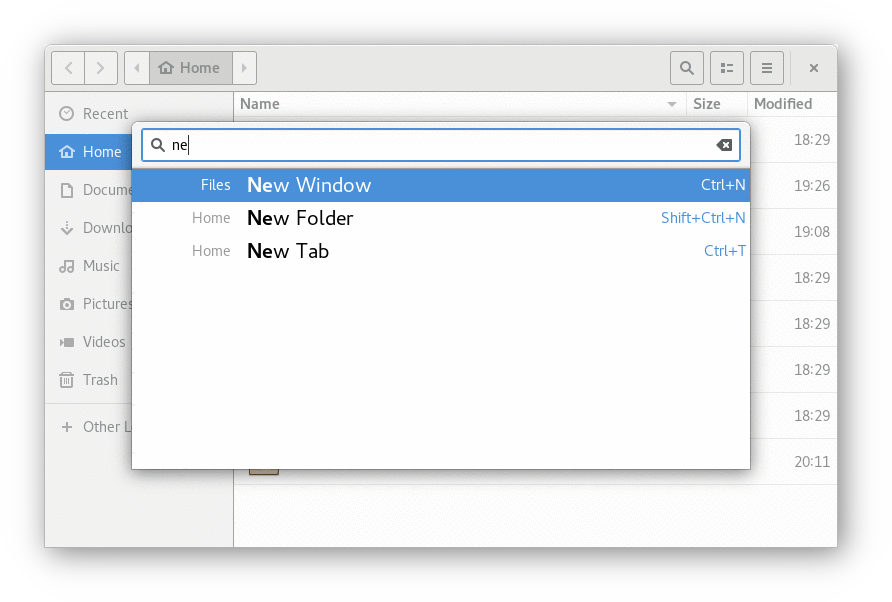
\includegraphics[height=0.9\textheight]{Plotinus}
\end{frame}

\begin{frame}{Фреймворк Qt}
    \begin{columns}
		\column{0.38\linewidth}
		\centering
		
\includegraphics[width=5cm]{Qt}
		\column{0.58\linewidth}
		\textbf{Qt}~— кроссплатформенный фреймворк для разработки программного обеспечения на языке программирования C++. Включает в себя в т.ч. классы для разработки
		графического интерфейса.
	\end{columns}
\end{frame}

\begin{frame}{Добавление функциональности в приложение}
	\textbf{Способы добавления дополнительной функциональности\\в приложение}
	\begin{itemize}
		\item Добавление функции на этапе сборки приложения
		\item Добавление функции в момент выполнения программы
		\begin{itemize}
			\item С помощью загрузка плагинов
			\item С помощью подмены библиотек
		\end{itemize}
	\end{itemize}
\end{frame}

\begin{frame}{Взаимодействие элементов GUI и пользователя}
	\begin{figure}
		\begin{tikzpicture}[
        ->,>=stealth',node
        distance=1.5cm, semithick,
        every edge/.append style={<->}
    ]

    \tikzstyle{block} = [rectangle,draw,minimum height=0.8cm]

    \node[block] (user) {Пользователь};
    \node[block] (x11) [below of=user] {Графическая подсистема X11};
    \node[block] (lib) [below of=x11] {Графическая библиотека Qt};
    \node[block] (app) [below of=lib] {Приложение};
    \path[]
        (user) edge (x11)
        (x11) edge (lib)
        (lib)  edge (app)
    ;

\end{tikzpicture}

	\end{figure}
\end{frame}

\begin{frame}{Внедрение библиотеки}
	\begin{figure}
		\begin{tikzpicture}[
        ->,>=stealth',node
        distance=1.5cm, semithick,
        every edge/.append style={<->}
    ]

    \tikzstyle{block} = [rectangle,draw,minimum height=0.8cm]
    \tikzstyle{bold} = [rectangle,draw,thick,minimum height=0.8cm,line width=1mm]

    \node[block] (user) {Пользователь};
    \node[block] (x11) [below of=user] {Графическая подсистема X11};
    \node[block] (lib) [below of=x11] {Графическая библиотека Qt};
    \node[bold] (inject) [below of=lib] {Внедряемый модуль};
    \node[block] (app) [below of=inject] {Приложение};
    \path[]
        (user)   edge (x11)
        (x11)    edge (lib)
        (lib)    edge (inject)
        (inject) edge (app)
    ;

\end{tikzpicture}

	\end{figure}
\end{frame}

\begin{frame}{Механизм подмены функций}
	\begin{figure}
		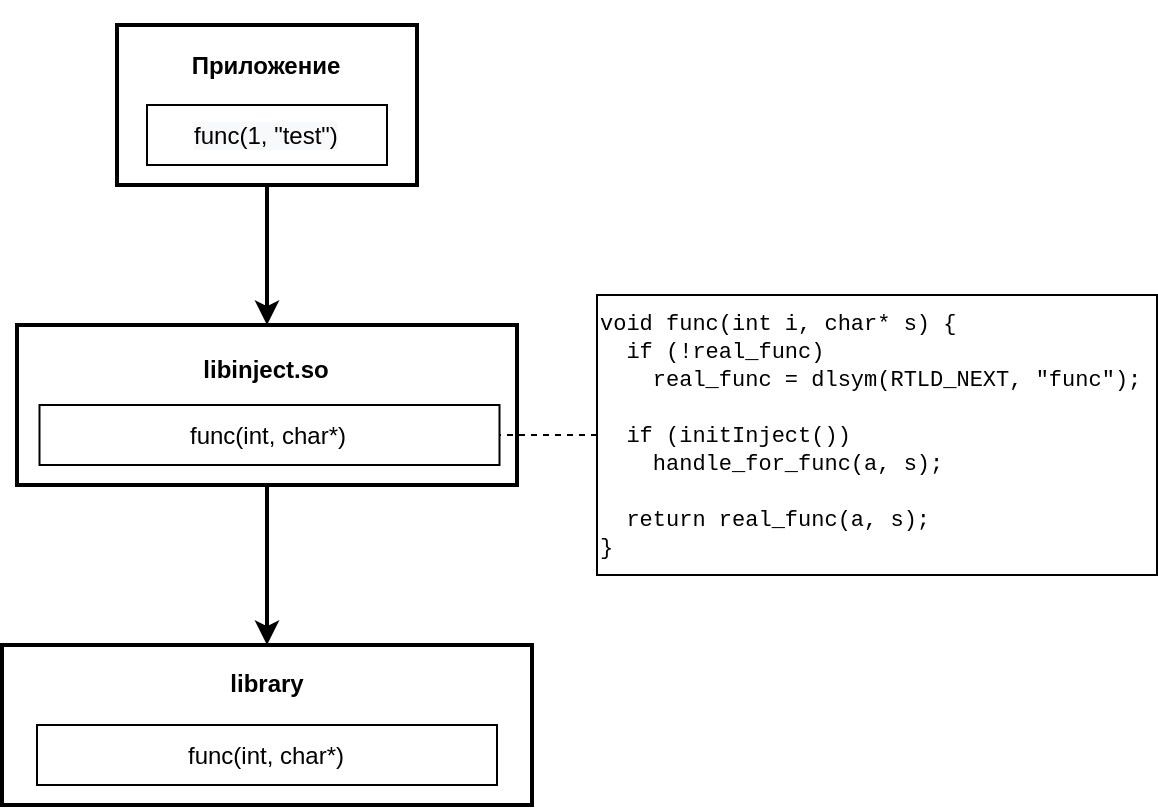
\includegraphics[height=0.8\textheight]{inject}
	\end{figure}
\end{frame}

\begin{frame}{Искажение имен}
	\begin{itemize}
		\item Было: \texttt{QCheckBox::QCheckBox(const QString\&, QWidget*)}
		\item Стало: \texttt{\_ZN9QCheckBoxC1ERK7QStringP7QWidget}
	\end{itemize}
	\vspace{0.7cm}
	\begin{itemize}
		\item Было: \texttt{void QAbstractButton::setText(const QString\&)}
		\item Стало: \texttt{\_ZN15QAbstractButton7setTextERK7QString}
	\end{itemize}
\end{frame}

\begin{frame}{Задачи реализации}
	Реализовать:
	\begin{itemize}
		\item Генератор кода функций-обработчиков
		\item Библиотеку для сбора информации
		\item Приложение для отображения палитры команд
	\end{itemize}
\end{frame}

\begin{frame}{Архитектура системы}
	\begin{figure}
		\centering
		\begin{tikzpicture}[
        ->,>=stealth',node
        distance=2cm, semithick
    ]

    \tikzstyle{block} = [rectangle,draw,minimum height=0.8cm]

    \node[block] (preload) {Подгружаемый модуль};
    \node[block] (lib)    [above of=preload] {libQtWidgets};
    \node[block] (x11)    [above of=lib]     {X11};
    \node[block] (server) [left=2cm of preload] {Сервер управления};
    \node[block] (app)    [below of=preload] {Целевое приложение};

    \node[block] (ctrl) [above of=server] {Приложение управления};
    \node[block] (user) [above of=ctrl] {Пользователь};

    \path[]
        (app)     edge[bend left]     node[left]  {1} (preload)
        (preload) edge[bend left=5]   node[below] {2} (server)
        (preload) edge[bend left]     node[left]  {3} (lib)
        (lib)     edge[bend left]     node[left]  {4} (x11)
        (server)  edge[bend left]     node[left]  {5} (ctrl)
        (ctrl)    edge[bend left]     node[left]  {6} (user)
        (user)    edge[bend left]     node[right] {7} (ctrl)
        (ctrl)    edge[bend left]     node[right] {8} (server)
        (server)  edge[bend left=5]   node[above] {9} (preload)

        (server.north east)  edge    node[above]{10} (x11)

        (x11)     edge[bend left]     node[right] {11} (lib)
        (lib)     edge[bend left]     node[right] {12} (preload)
        (preload) edge[bend left]     node[right] {13} (app)
        (preload) edge[bend right=75] node[right] {14} (lib)
        (lib)     edge[bend left=80]  node[right]  {15} (app)
    ;

\end{tikzpicture}

	\end{figure}
\end{frame}

\begin{frame}[fragile]{Протокол}
	\begin{minted}{text}
    <команда> ::= <имя-­команды> <параметры-­команды>
    <имя-­команды> ::= <строка>
    <строка> ::= <длина-­строки> <идентификатор>
    <длина-­строки> ::= uint32_t
    <идентификатор> ::= "newApp"
                    ::= "setWidgetText"
                    ::= "remove"
                    ::= "activated"
                    ::= "setWidgetWindow"
                    ::= "activate"
	\end{minted}
\end{frame}

\iffalse
\begin{frame}{Приложение управления}
	\centering
	\input{../schemes/app_arch.tex}
\end{frame}
\fi

\iffalse
\begin{frame}{Интерфейс}
    \begin{columns}
		\column{0.58\linewidth}
		Сочетания клавиш
		\begin{itemize}
			\item Запуск: Ctrl + Shift + D
			\item Палитра: Ctrl + Shift + S
		\end{itemize}
		\column{0.38\linewidth}
		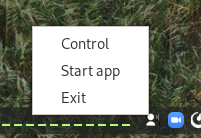
\includegraphics[width=3cm]{tray_ui}
	\end{columns}
\end{frame}
\fi

\forloop{example}{0}{\value{example} < 5}%
{
	\begin{frame}{Интерфейс}
		\centering
		\includegraphics[height=0.9\textheight]{example\theexample}
	\end{frame}
}

\begin{frame}{Заключение}
	\begin{itemize}
		\item Выбран подходящий способ добавления функции в приложение
		\item Реализован генератор кода
		\item Реализована внедряемая библиотека, для сбора информации\\
		об элементах интерфейса
		\item Реализовано приложение для отображения палитры команд
	\end{itemize}
\end{frame}

\begin{frame}[plain]
	\titlepage
\end{frame}

\end{document}
